\hypertarget{what-is-iot}{%
\section{What is IoT}\label{what-is-iot}}

\begin{frame}{What is IoT}
\protect\hypertarget{what-is-iot-1}{}

\begin{itemize}
\tightlist
\item
  Not “a computer connected to the internet”

  \begin{itemize}
  \tightlist
  \item
    Then it is really just another computer connected to the internet
  \end{itemize}
\item
  Must be something else

  \begin{itemize}
  \tightlist
  \item
    It is simply devices that are resource constrained

    \begin{itemize}
    \tightlist
    \item
      Usually in more than one way
    \end{itemize}
  \end{itemize}
\item
  Autonomous operation, the connection might not be permanent
\end{itemize}

\end{frame}

\begin{frame}{IoT is just a concept}
\protect\hypertarget{iot-is-just-a-concept}{}

\begin{itemize}
\tightlist
\item
  \emph{The Internet of Things (IoT) is the network of physical devices,
  vehicles, home appliances and other items embedded with electronics,
  software, sensors, actuators, and connectivity which enables these
  objects to connect and exchange data.}\footnote<.->{Wikipedia
    “Internet of Things”}
\end{itemize}

\end{frame}

\begin{frame}{What is an IoT Device?}
\protect\hypertarget{what-is-an-iot-device}{}

\begin{itemize}
\tightlist
\item
  Constrained in (one or more of):

  \begin{itemize}
  \tightlist
  \item
    Memory
  \item
    CPU
  \item
    Network bandwidth and/or latency
  \item
    Storage
  \end{itemize}
\end{itemize}

\note{What differentiates a computer from an IoT device?}

\end{frame}

\hypertarget{going-back-to-basics}{%
\section{Going back to basics}\label{going-back-to-basics}}

\begin{frame}{What is the internet again?}
\protect\hypertarget{what-is-the-internet-again}{}

\end{frame}

\begin{frame}{OSI model}
\protect\hypertarget{osi-model}{}

\begin{enumerate}
[1.]
\tightlist
\item
  Physical Layer
\item
  Data Link Layer
\item
  Network Layer
\item
  Transport Layer
\item
  Session Layer
\item
  Presentation Layer
\item
  Application Layer
\end{enumerate}

\begin{itemize}
\tightlist
\item
  \href{https://en.wikipedia.org/wiki/OSI_model}{Wikipedia: OSI model}
\item
  \href{https://en.wikipedia.org/wiki/OSI_model\#Examples}{Wikipedia:
  OSI model\#Examples}
\end{itemize}

\note{Does not match the TCP/IP stack very closely.}

\end{frame}

\begin{frame}{Layer 1: Physical Layer}
\protect\hypertarget{layer-1-physical-layer}{}

\begin{itemize}
\tightlist
\item
  10BASE5, 10BASE2
\item
  10BASE-T / 100BASE-TX / 1000BASE-TX
\item
  802.11a/b/g/n PHY
\item
  RS-232
\end{itemize}

\note{Ethernet: Hubs and switches (that act on this level) is not on
it’s own layer. It is more of a implementation detail in the
architecture diagram.

RS-232 signaling is used in \emph{all} MCUs, many have several ports
available. It is extremely flexible, both used for implementing
applications and debugging. Frequently an easy way to hack embedded
devices. “USB dongles”, “USB TTL” all use RS-232 signaling.

Note that this only applies to its logical signals, not voltage levels.
The signaling does not specify any max data rate, very high rates
(\textgreater{}= 1Mbps) is often supported.}

\end{frame}

\begin{frame}{Layer 2: Data Link Layer}
\protect\hypertarget{layer-2-data-link-layer}{}

\begin{itemize}
\tightlist
\item
  Ethernet
\item
  WiFi
\item
  Bluetooth
\item
  Token Ring
\end{itemize}

\end{frame}

\begin{frame}{Layer 3: Network Layer}
\protect\hypertarget{layer-3-network-layer}{}

\begin{itemize}
\tightlist
\item
  IP
\item
  ICMP
\item
  IPX
\end{itemize}

\end{frame}

\begin{frame}{Layer 4: Transport Layer}
\protect\hypertarget{layer-4-transport-layer}{}

\begin{itemize}
\tightlist
\item
  TCP
\item
  UDP
\end{itemize}

\end{frame}

\begin{frame}{Layer 5: Session Layer}
\protect\hypertarget{layer-5-session-layer}{}

\begin{itemize}
\tightlist
\item
  “sockets”
\item
  NetBIOS
\end{itemize}

\end{frame}

\begin{frame}{Layer 6: Presentation Layer}
\protect\hypertarget{layer-6-presentation-layer}{}

\begin{itemize}
\tightlist
\item
  SSL
\end{itemize}

\note{This layer is not really much used in the IP stack}

\end{frame}

\begin{frame}{Layer 7: Application Layer}
\protect\hypertarget{layer-7-application-layer}{}

\begin{itemize}
\tightlist
\item
  HTTP
\item
  MQTT
\item
  DNS
\item
  (everything else..)
\end{itemize}

\end{frame}

\begin{frame}{Details: IP}
\protect\hypertarget{details-ip}{}

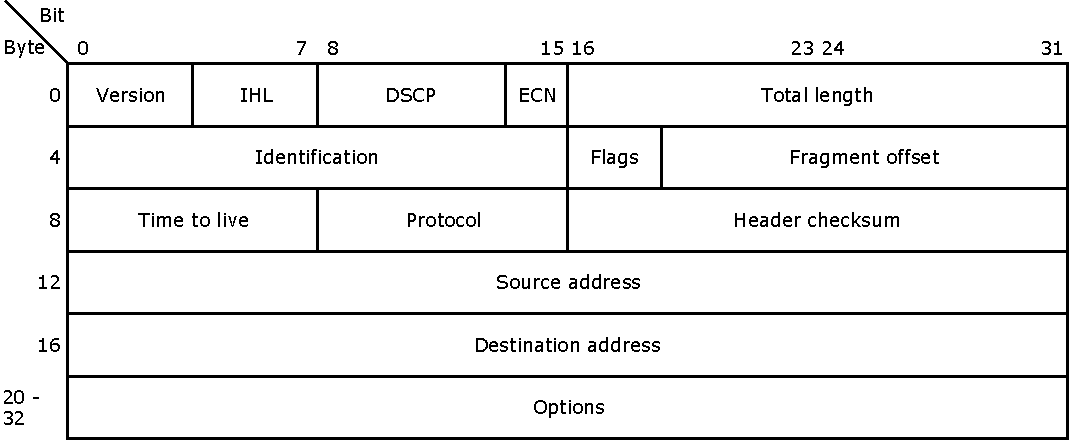
\includegraphics{images/ip-header.pdf}

\note{Note that the “total length” field is 16 bits, 2 bytes, it’s
maximum value is 64k, 65536.}

\end{frame}

\begin{frame}{Details: IP}
\protect\hypertarget{details-ip-1}{}

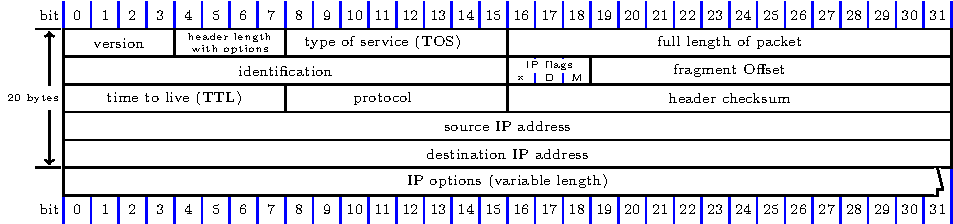
\includegraphics{images/IP-Header_eng.pdf}

\end{frame}

\hypertarget{notes}{%
\section{Notes}\label{notes}}

\begin{frame}{Assignments}
\protect\hypertarget{assignments}{}

\begin{itemize}
\tightlist
\item
  Measure round trip time/latency. Measure UDP, TCP. Measure when the
  packet size is greater than the MTU
\end{itemize}

\end{frame}
